%# -*- coding: utf-8 -*-
% xiantu.tex
% asymptotebyexample 的一章,最基础的画图知识

\chapter{赵爽的弦图}
\label{chap:xiantu}

赵爽博士是位老知识分子,研究兴趣是天文历法与算学,一生精研《周髀算经》。不过
赵老爷子年轻的时候书籍都是手写,最近才紧跟时代潮流用上了电脑。现在他要修订他
研究《周髀算经》的札记,决定使用 \LaTeX{} 来排版。

现在他遇到一个难题,就是他要画出笔记中讲解勾股定理的一幅弦图。听人介绍,几经
比较之后,他决定使用现在炒得火热的 \Asy{}。

赵博士的原图是手画的,线框多有不直不准的,\autoref{fig:xiantuancient} 就是旧
年据手稿做的雕版图,赵博士并不满意。赵爽博士理想中的图,线条要平整美观,文字
要清楚整齐,图形还要上色:朱实自然得用红色,黄实也该用黄色,以与注文一致——
就是\autoref{fig:xiantu} 的样子。

\begin{figure}
  \centering
  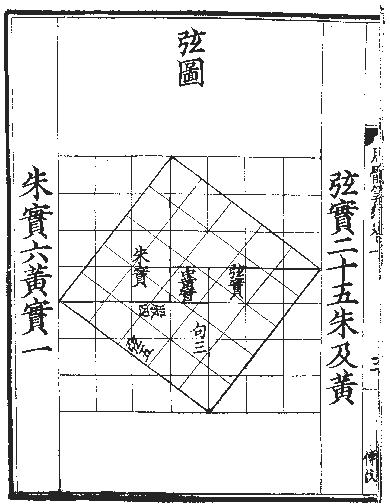
\includegraphics[height=\textheight-2\baselineskip]{xiantu-ancient.pdf}
  \caption{旧年做的雕版}
  \label{fig:xiantuancient}
\end{figure}
\begin{figure}
  \centering
  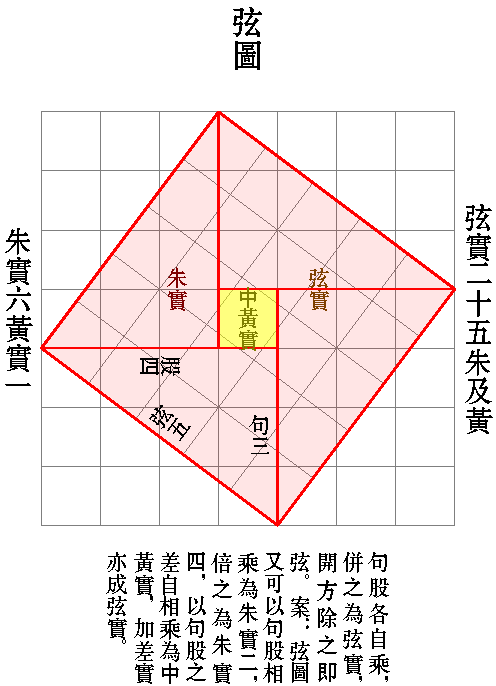
\includegraphics{xiantu.pdf}
  \caption{理想中的新版本}
  \label{fig:xiantu}
\end{figure}

计议已定,赵博士要开始正式的绘图了。

\section{绘图环境}

\Asy{} 的安装并不复杂,在 Windows 下面就是下载运行那个安装包,在 Linux 下面一
般也只需要下载对应的压缩包,解压就可以使用了。哦,赵博士用的就是 Windows。

点图标运行 \Asy{},就出现了交互式\index{交互式}的命令行,提示符是一个
\verb=>=。输入命令:
\begin{lstlisting}
draw((0,0) -- (3cm,4cm));   // `\color{comment}一条直线`
\end{lstlisting}
赵博士装的 GSView 立即弹了出来,里面已经画出一条倾斜的直线。再输入
|quit|\index{quit@\lstinline=quit=},程序退出,并留下了一个叫做
\verb=out.eps= 的图形文件,
小菜一碟。

这里稍稍解释一下上面的一句代码。|draw|\index{draw@\lstinline=draw=} 是画线的
命令,更准确地说,是 \Asy{} 中的函数\index{函数}:它带有一个参数\index{参数}
|(0,0) -- (3cm,4cm)|,参数外面是圆括号,整个命令以分号结束。里面的
|(0,0) -- (3cm,4cm)| 是由两个坐标\index{坐标}连接而成的直线,坐标是在直角坐标
系下的,可以带单位 |mm|, |cm|, |pt|, |bp|, |inch|, |inches|,%
\index{mm@\lstinline=mm=}\index{cm@\lstinline=cm=}\index{pt@\lstinline=pt=}%
\index{bp@\lstinline=bp=}\index{inch@\lstinline=inch=}%
\index{inches@\lstinline=inches=}%
其意义与在\TeX{} 中的一样,如果不带单位,则默认为 |bp|。行末以 |//| 开头的是
注释,另有一种在 |/* */| 之间的注释\index{注释},与 C 语言相同。

\index{编译}
不过赵博士写书讲求胸有成竹方才下笔,因此他更愿意使用更一种方式:打开一个文本
编辑器,把上面的绘图命令都录入完毕,保存为一个名为 \verb=line.asy= 的文件,最
后把这个文件拖动到 \Asy{} 的图标上面,就完成了整个作图。

赵博士的小侄子不屑于这种快捷图标的编译方式,他直接进入命令行,输入
\verb=asy=,就进入了 \Asy{} 的交互环境;要是输入 \verb=asy line=,就画出了刚
才的保存的直线。


\section{直线与绘图命令}
\label{sec:linedraw}

弦图的图形其实很简单,都是直线、方块、三角形这些,而且为了计算的简便,所有长
度也都是整数值。那么,首先就是在 \Asy{} 中来画直线。

\index{画线}
正如前面试验的时候做的那样,一条直线就是用 |--|\index{--@\lstinline=--=} 把坐
标连起来,再使用 |draw| 命令,直线就画出来了。事实上,可以用 |--| 把坐标点连
成折线:
\begin{lstlisting}
draw( (0,0) -- (1cm,0) -- (2cm,0.5cm) -- (1cm,1cm) -- (0,1cm) );
\end{lstlisting}
\begin{figure}[H]
\centering
\begin{asy}
draw( (0,0) -- (1cm,0) -- (2cm,0.5cm) -- (1cm,1cm) -- (0,1cm) );
\end{asy}
\end{figure}

像这样把坐标用 |--| 连结起来的,就成为一条路径\index{路径}。把直线而稍做修改
,在后面连上一个特殊的坐标 |cycle|\index{cycle@\lstinline=cycle=},就可以得到
一条首尾相接的闭路径\index{路径!闭路径}。如:
\begin{lstlisting}
draw( (0,0) -- (1cm,0) -- (2cm,0.5cm) -- (1cm,1cm) -- (0,1cm) -- cycle );
\end{lstlisting}
\begin{figure}[H]
\centering
\begin{asy}
draw( (0,0) -- (1cm,0) -- (2cm,0.5cm) -- (1cm,1cm) -- (0,1cm) -- cycle );
\end{asy}
\end{figure}

画一条路径可以使用不同的颜色、粗细的笔,这只要给 |draw| 命令多加一个画笔
\index{画笔}参数(多个参数用逗号分开):
\begin{lstlisting}
draw((0,0) -- (1cm,0) -- (2cm,0.5cm) -- (1cm,1cm) -- (0,1cm), darkblue+1mm);
\end{lstlisting}
\begin{figure}[H]
\centering
\begin{asy}
draw((0,0) -- (1cm,0) -- (2cm,0.5cm) -- (1cm,1cm) -- (0,1cm), darkblue+1mm);
\end{asy}
\end{figure}
这里 |darkblue| 是颜色,|1mm| 是线的粗细。|darkblue+1mm| 即指一毫米宽的深
蓝色粗线。(可用的颜色\index{颜色}名称可以参考 \cite{asyman})

赵博士画的是“勾三股四弦五”的红色三角形,这很容易:
\begin{lstlisting}
draw( (0,0) -- (4cm,0) -- (0,3cm) -- cycle, red+0.5mm );
\end{lstlisting}
\begin{figure}[H]
\centering
\begin{asy}
draw( (0,0) -- (4cm,0) -- (0,3cm) -- cycle, red+0.5mm );
\end{asy}
\end{figure}

\index{填充}
不过现在还需要的是实心的三角形,因此就需要一个新的绘图命令
|fill|\index{fill@\lstinline=fill=},即填充。于是,红色三角形就成为
\begin{lstlisting}
fill( (0,0) -- (4cm,0) -- (0,3cm) -- cycle, red );
\end{lstlisting}
\begin{figure}[H]
\centering
\begin{asy}
fill( (0,0) -- (4cm,0) -- (0,3cm) -- cycle, red );
\end{asy}
\end{figure}

但这样一来三角形的颜色就太重了,而且边界也不清楚。因此似乎应该先用浅红色填充
一遍,然后再用深红色勾边。好在可以使用一个命令
|filldraw|\index{filldraw@\lstinline=filldraw=} 同时完成这两件事情,这样就不
需要把一条路径写两遍了。即有:
\begin{lstlisting}
filldraw((0,0) -- (4cm,0) -- (0,3cm) -- cycle,
    fillpen=palered, drawpen=red+0.5mm);
\end{lstlisting}
\begin{figure}[H]
\centering
\begin{asy}
filldraw((0,0) -- (4cm,0) -- (0,3cm) -- cycle,
    fillpen=palered, drawpen=red+0.5mm);
\end{asy}
\end{figure}
这里可以简单地直接写两个参数 |palered, red+0.5mm|,不过为了清晰起见还是使用
“$\text{键}=\text{值}$”的写法,明确表示出填充的画笔和描线的画笔。

现在,赵博士的整个弦图的框架就呼之欲出了,就是画出四个三角形
(\autoref{fig:xiantuskeleton}):
\begin{lstlisting}
filldraw( (4cm,0) -- (4cm,3cm) -- (0,3cm) -- cycle,
    fillpen=palered, drawpen=red+0.5mm);
filldraw( (7cm,4cm) -- (4cm,4cm) -- (4cm,0) -- cycle,
    fillpen=palered, drawpen=red+0.5mm);
filldraw( (3cm,7cm) -- (3cm,4cm) -- (7cm,4cm) -- cycle,
    fillpen=palered, drawpen=red+0.5mm);
filldraw( (0,3cm) -- (3cm,3cm) -- (3cm,7cm) -- cycle,
    fillpen=palered, drawpen=red+0.5mm);
\end{lstlisting}
\begin{figure}
\centering
\begin{asy}
filldraw( (4cm,0) -- (4cm,3cm) -- (0,3cm) -- cycle,
    fillpen=palered, drawpen=red+0.5mm);
filldraw( (7cm,4cm) -- (4cm,4cm) -- (4cm,0) -- cycle,
    fillpen=palered, drawpen=red+0.5mm);
filldraw( (3cm,7cm) -- (3cm,4cm) -- (7cm,4cm) -- cycle,
    fillpen=palered, drawpen=red+0.5mm);
filldraw( (0,3cm) -- (3cm,3cm) -- (3cm,7cm) -- cycle,
    fillpen=palered, drawpen=red+0.5mm);
\end{asy}
\caption{弦图的初步框架}\label{fig:xiantuskeleton}
\end{figure}

还应该画出弦图的中间的“黄实”,用黄色填充。这部分是一个正方形,可以使用现成
的 \lstinline[mathescape]|box($\text{角点}$, $\text{角点}$)|
\index{box@\lstinline=box=} 命令来产生矩形的路径,因而填充正中间的正方形就可
以用:
\begin{lstlisting}
fill( box((3cm,3cm), (4cm,4cm)), yellow );
\end{lstlisting}
这个填充的命令应该放在画线之前(以免覆盖描的红线)。

回顾前面的代码,赵博士觉得连续地写四个 |filldraw| 命令太重复了。他读了 \Asy{}
的文档 \cite{asyman},才知道多条路径可以用符号 |^^|\index{^^@\lstinline=^^=} 
连起来,一起使用,于是立即着手改进原来的代码。

而且,由于还打算在图的后面画出参考网格,图形的颜色还应该设置为半透明\index{透
明}的。好在这并不难实现,只要稍稍改动一下填充的画笔,使用
\lstinline[mathescape]|opacity($\text{数值}$)|
\index{opacity@\lstinline=opacity=}
来设定有一定不透明度(取值为 $0\sim1$)的画笔,并把它加在原来的画笔上
\footnote{\Asy{} 的 EPS 格式输出看不到透明效果,必须输出为 PDF 格式或从 PDF 
格式转化为其他格式才能有透明效果。}。于是赵博士最后写出了这样的代码:
\begin{lstlisting}
fill( box((3cm,3cm), (4cm,4cm)), opacity(0.5)+yellow );
filldraw( (4cm,0) -- (4cm,3cm) -- (0,3cm) -- cycle
    ^^ (7cm,4cm) -- (4cm,4cm) -- (4cm,0) -- cycle
    ^^ (3cm,7cm) -- (3cm,4cm) -- (7cm,4cm) -- cycle
    ^^ (0,3cm) -- (3cm,3cm) -- (3cm,7cm) -- cycle,
    fillpen=opacity(0.1)+red, drawpen=red+0.5mm );
\end{lstlisting}
至此,弦图的主要框架(\autoref{fig:xiantuskeleton2})就此完成。
\begin{figure}[H]
\centering
\begin{asy}
fill( box((3cm,3cm), (4cm,4cm)), opacity(0.5)+yellow );
filldraw( (4cm,0) -- (4cm,3cm) -- (0,3cm) -- cycle
    ^^ (7cm,4cm) -- (4cm,4cm) -- (4cm,0) -- cycle
    ^^ (3cm,7cm) -- (3cm,4cm) -- (7cm,4cm) -- cycle
    ^^ (0,3cm) -- (3cm,3cm) -- (3cm,7cm) -- cycle,
    fillpen=opacity(0.1)+red, drawpen=red+0.5mm );
\end{asy}
\caption{弦图的进一步优化的框架}\label{fig:xiantuskeleton2}
\end{figure}


\section{图形变换与功能模块的使用}
\label{sec:transformmodule}

然后是画作为长度参考的网格。其实网格一开始就该在图中画出来,这样后面画图准确
与否才能看得清楚。不过现在赵博士是重作旧图,图样已定,网格就搁在弦图的主要图
形后面才画了。

按说这个网格是十分简单的,无非就是画一些灰色的纵横细线。比如这个 $3\times3$ 
的网格:
\begin{lstlisting}
draw( (0,0) -- (3cm,0)
    ^^ (0,1cm) -- (3cm,1cm)
    ^^ (0,2cm) -- (3cm,2cm)
    ^^ (0,3cm) -- (3cm,3cm),
    gray );
draw( (0,0) -- (0,3cm)
    ^^ (1cm,0) -- (1cm,3cm)
    ^^ (2cm,0) -- (2cm,3cm)
    ^^ (3cm,0) -- (3cm,3cm),
    gray );
\end{lstlisting}
\begin{figure}[H]
\centering
\begin{asy}
draw( (0,0) -- (3cm,0)
    ^^ (0,1cm) -- (3cm,1cm)
    ^^ (0,2cm) -- (3cm,2cm)
    ^^ (0,3cm) -- (3cm,3cm),
    gray );
draw( (0,0) -- (0,3cm)
    ^^ (1cm,0) -- (1cm,3cm)
    ^^ (2cm,0) -- (2cm,3cm)
    ^^ (3cm,0) -- (3cm,3cm),
    gray );
\end{asy}
\end{figure}

可无疑这个办法显得太麻烦了,赵博士要画的是 $7\times7$ 的网格,就要分别画出
$16$ 条直线。这样的代码不仅不好写,而且容易出错,修改一下也很麻烦。

赵博士看到了手册 \cite{asyman} 中讲循环语句的用法,似乎可以完成这件事。可是以
赵博士的年龄,再去看什么编程什么变量的,命令不能一条一条执行下来,很不习惯,
头脑就往往转不清楚。

\index{模块!math@\prgname{math}}
于是赵博士就去论坛上咨询,一些人劝他去用几行循环语句,甚至有人已经把完整的函
数做好了。但有一个结果特别引人注目,有人指出,在 \prgname{math} 模块中已经定
义好了一个 |grid| 函数,只要拿来用就可以了。赵博士立即精神大振,来看这个
|grid| 函数:\index{grid@\lstinline=grid=}
\begin{lstlisting}
picture grid(int Nx, int Ny, pen p=currentpen)
\end{lstlisting}
这个是在 \prgname{math} 模块中 |grid| 函数的原型。\index{原型}它说明 |grid| 
函数有 |Nx|, |Ny| 两个整数类型的必需参数,一个可选的画笔,并且返回一个
|picture|(图)\index{picture@\lstinline=picture=}类型的对象。

\index{导入}\index{模块!导入}
要使用模块的功能,需要在绘图之前导入这个模块,这只要使用
\index{import@\lstinline=import=}
\begin{lstlisting}
import `模块名`;
\end{lstlisting}
因此,要使用 \prgname{math} 模块中的 |grid| 函数,只要在代码中写
\begin{lstlisting}
import math;
\end{lstlisting}
就可以了。

|grid| 函数的行为看起来很奇怪,调用它会在一个单独的图上画出一个
|Nx|${}\times{}$|Ny| 的网格,网格的左下角在原点,间距为 $1$。要使用 |grid| 函
数画的图形,要使用 \lstinline[mathescape]|add($\text{图}$)|
\index{add@\lstinline=add=} 命令,把这个图形加在当前的图上:
\begin{lstlisting}
import math;
add(grid(10,10,gray));
\end{lstlisting}
\begin{figure}[H]
\centering
\begin{asy}
import math;
add(grid(10,10,gray));
\end{asy}
\end{figure}
不过直接这样做的结果是只能得到一个小得已经看不清的网格。因此,必须对图形进行放缩。

\index{变换}\index{仿射变换}
\index{变换!平移}\index{变换!旋转}\index{变换!放缩}
\index{变换!错切}\index{变换!反射}
\Asy{} 提供了平移、旋转、放缩、倾斜、反射等各种的仿射变换,来对坐标、路径、图
形等元素进行变换(严格的函数原型参考 \cite{asyman}):
\index{shift@\lstinline=shift=}
\index{scale@\lstinline=scale=}
\index{xscale@\lstinline=xscale=}
\index{yscale@\lstinline=yscale=}
\index{rotate@\lstinline=rotate=}
\index{slant@\lstinline=slant=}
\index{reflect@\lstinline=reflect=}
\begin{lstlisting}
shift(`坐标`)           // `\color{comment}按坐标平移`
shift(x, y)           // `\color{comment}按` (x, y) `\color{comment}平移`
scale(`倍数`)           // `\color{comment}按倍数放缩`
xscale(`倍数`)          // `\color{comment}$x$ 轴方向按倍数放缩`
yscale(`倍数`)          // `\color{comment}$y$ 轴方向按倍数放缩`
scale(x, y)           // `\color{comment}在 $x$ 轴、$y$ 轴方向分别按倍数` x, y `\color{comment}放缩`
rotate(`角度`, z=(0,0)) // `\color{comment}按角度绕中心` z`\color{comment}(默认为原点,逆时针)旋转`
slant(`因子`)           // `\color{comment}按一定因子向右倾斜`
reflect(a, b)         // `\color{comment}相对直线` a--b `\color{comment}反射`
\end{lstlisting}
使用一个变换就是把这个变换乘在被变换对象的左边。例如一个放缩一个单位正方形:
\begin{lstlisting}
draw( scale(2cm) * box((0,0), (1,1)) );
\end{lstlisting}
\begin{figure}[H]
\centering
\begin{asy}
draw( scale(2cm) * box((0,0), (1,1)) );
\end{asy}
\end{figure}
这样的变换可以连续地做下去,例如
\begin{lstlisting}
draw( rotate(90) * slant(0.3) * scale(1cm) * box((0,0), (1,1)) );
\end{lstlisting}
就是把一个单位正方形先放大,再倾斜,再旋转 $90^\circ$:
\begin{figure}[H]
\centering
\begin{asy}
draw( rotate(90) * slant(0.3) * scale(1cm) * box((0,0), (1,1)) );
\end{asy}
\end{figure}

有了这些变换,画出一个合适大小的网格就不再是什么难事了:
\begin{lstlisting}
import math;
add( scale(5mm) * grid(4, 4, gray) );
\end{lstlisting}
\begin{figure}[H]
\centering
\begin{asy}
import math;
add( scale(5mm) * grid(4, 4, gray) );
\end{asy}
\end{figure}

赵博士的弦图有两个网格,不仅要大小合适,而且其中一个需要进行旋转和平移。平移
的位置很明显,但旋转仍然需要一些计算。当然这难不倒精研天文算学多年的赵博士,
这里弦实($5\times5$ 的正方形)可以看作是顺时针旋转得到的,从朱实的三角形容易
看出旋转的角度正好是 $\arctan(3/4)$。\Asy{} 中也可以方便地调用返回角度的反三
角函数 |aTan|\index{aTan@\lstinline=aTan=} 来计算这个角度\footnote{也可以使用
atan2 函数,但注意返回值是弧度。}。更详细的数学函数列表,参看 \cite{asyman}。
(注意:C/C++ 中 |3/4| 表示求带余除法 $3\div 4$ 的商,得到 $0$;但在 \Asy{} 中
|3/4| 的结果是实数 $0.75$,整数的带余除法则用 |quotient(a,b)|
\index{quotient@\lstinline=quotient=} 函数。)

于是,赵博士弦图中的网格,就可以这样方便地画出来了
(\autoref{fig:xiantugrid}):
\begin{lstlisting}
// `\color{comment}网格`
import math;
add( scale(1cm) * grid(7, 7, gray) );
add( shift(0,3cm) * rotate(-aTan(3/4)) * scale(1cm) * grid(5, 5, gray) );
// `\color{comment}弦图主体`
fill( box((3cm,3cm), (4cm,4cm)), opacity(0.5)+yellow );
filldraw( (4cm,0) -- (4cm,3cm) -- (0,3cm) -- cycle
    ^^ (7cm,4cm) -- (4cm,4cm) -- (4cm,0) -- cycle
    ^^ (3cm,7cm) -- (3cm,4cm) -- (7cm,4cm) -- cycle
    ^^ (0,3cm) -- (3cm,3cm) -- (3cm,7cm) -- cycle,
    fillpen=opacity(0.1)+red, drawpen=red+0.5mm );
\end{lstlisting}
\begin{figure}[htbp]
\centering
\begin{asy}
// 网格
import math;
add( scale(1cm) * grid(7, 7, gray) );
add( shift(0,3cm) * rotate(-aTan(3/4)) * scale(1cm) * grid(5, 5, gray) );
// 弦图主体
fill( box((3cm,3cm), (4cm,4cm)), opacity(0.5)+yellow );
filldraw( (4cm,0) -- (4cm,3cm) -- (0,3cm) -- cycle
    ^^ (7cm,4cm) -- (4cm,4cm) -- (4cm,0) -- cycle
    ^^ (3cm,7cm) -- (3cm,4cm) -- (7cm,4cm) -- cycle
    ^^ (0,3cm) -- (3cm,3cm) -- (3cm,7cm) -- cycle,
    fillpen=opacity(0.1)+red, drawpen=red+0.5mm );
\end{asy}
\caption{带网格的弦图草图}
\label{fig:xiantugrid}
\end{figure}


\section{标注文字}

\index{标注}\index{标签}
现在要进行的是文字的标注。按照勾股定理的约定,赵博士打算在一个红色三角形内标
注“朱实”,在黄色矩形处标注“黄实”,并为拼得的整个大矩形标注“弦实”;在另
一红色三角形的三边标注“勾三”、“股四”、“弦五”的尺寸;最后在图形两侧加上
说明的文字。

在标注文字之前,对于中文标签\index{标签!中文标签},应该先定义好中文环境和字体
。\Asy{} 会调用 \LaTeX{} 来进行标签的处理,因而需要设置的就是 \LaTeX{} 的编译
引擎\index{LaTeX@\LaTeX!引擎}与一般的中文 \LaTeX{} 文件导言区。在这里,赵博士决定使
用 \XeTeX{}\index{XeTeX@\XeTeX} 引擎与
\prgname{xeCJK}\index{xeCJK@\prgname{xeCJK}} 宏包来处理中文。为此,在 \Asy{} 
源文件中,他使用了下面的设置代码:
\begin{lstlisting}
settings.tex = "xelatex";
usepackage("xeCJK");
texpreamble("\setCJKmainfont{SimSun}");
\end{lstlisting}
这里第一行是设置编译时所用的 \TeX{} 引擎。后面
|usepackage|\index{usepackage@\lstinline=usepackage=} 命令就是 \LaTeX{} 中的
\texcode|\usepackage| 命令的一个包装形式,里面的字符串参数就是宏包名;而
|texpreamble|\index{texpreamble@\lstinline=texpreamble=} 命令则把接收的参数直
接放进 \LaTeX{} 的导言区。

进行上述设置后,就可以正确使用中文标签了。标注的命令很简单,就是
|label|\index{label@\lstinline=label=},参数正是标签文字和标签的位置。例如:
\begin{lstlisting}
draw( (0,0) -- (1cm,1cm) -- (2cm,0) );
label( "`\color{string}中间`", (1cm,0cm) );
\end{lstlisting}
就得到
\begin{figure}[H]
\centering
\begin{asy}
settings.tex = "xelatex";
usepackage("xeCJK");
texpreamble("\setCJKmainfont{SimSun}");
draw( (0,0) -- (1cm,1cm) -- (2cm,0) );
label( "中间", (1cm,0cm) );
\end{asy}
\end{figure}

可以在标签中使用任意的 \LaTeX{} 代码,包括数学公式,例如:
\begin{lstlisting}
label("$x = \sin\alpha$", (0,0));
\end{lstlisting}
就会正确地得到 $x = \sin\alpha$ 的标签。

现在,我们可以给弦图加上“朱实”、“黄实”和“弦实”的标签了。在前面的框架代
码后面加上
\begin{lstlisting}
label("`\color{string}朱实`", (2cm,4cm));
label("`\color{string}黄实`", (3.5cm,3.5cm));
label("`\color{string}弦实`", (5cm,4cm));
\end{lstlisting}
以及设置字体的代码,就得到\autoref{fig:xiantupartlabel} 的结果。
\begin{figure}
\centering
\begin{asy}
settings.tex = "xelatex";
usepackage("xeCJK");
texpreamble("\setCJKmainfont{SimSun}");
import math;
add( scale(1cm) * grid(7, 7, gray) );
add( shift(0,3cm) * rotate(-aTan(3/4)) * scale(1cm) * grid(5, 5, gray) );
fill( box((3cm,3cm), (4cm,4cm)), opacity(0.5)+yellow );
filldraw( (4cm,0) -- (4cm,3cm) -- (0,3cm) -- cycle
    ^^ (7cm,4cm) -- (4cm,4cm) -- (4cm,0) -- cycle
    ^^ (3cm,7cm) -- (3cm,4cm) -- (7cm,4cm) -- cycle
    ^^ (0,3cm) -- (3cm,3cm) -- (3cm,7cm) -- cycle,
    fillpen=opacity(0.1)+red, drawpen=red+0.5mm );
label("朱实", (2cm,4cm));
label("黄实", (3.5cm,3.5cm));
label("弦实", (5cm,4cm));
\end{asy}
\caption{带部分标注的弦图}\label{fig:xiantupartlabel}
\end{figure}

下面则是要给三角形的三边进行标注。

\index{标签!路径上的标签}
与前面在一个点处标注不同,这里实际是给一条路径(直线)标注标签。因此,想要得
到的是距离这条路径的中点一定方向距离加一个标签,而不是简单地取路径上的一点作
为标签的位置。好在 \Asy{} 确实也提供了这样的功能,仍然使用 |label| 命令,基本
语法是:\index{label@\lstinline=label=}
\begin{lstlisting}
label(`标签`, `路径`)
\end{lstlisting}
这里默认会在路径中间的右侧(沿着路径行进方向)加标签。例如:
\begin{lstlisting}
draw( (0,0) -- (4cm,2cm), linewidth(0.5mm) );
label("`\color{string}粗线条`", (0,0) -- (4cm,2cm));
\end{lstlisting}
(其中的 |linewidth|\index{linewidth@\lstinline=linewidth=} 函数用来表示具有
一定线宽\index{线宽}的画笔)这段代码将得到
\begin{figure}[H]
\centering
\begin{asy}
settings.tex = "xelatex";
usepackage("xeCJK");
texpreamble("\setCJKmainfont{SimSun}");
draw( (0,0) -- (4cm,2cm), linewidth(0.5mm) );
label("粗线条", (0,0) -- (4cm,2cm));
\end{asy}
\end{figure}

现在,赵博士就可以给三角形的三边加上“勾三”、“股四”、“弦五”的标签了,只
要稍稍注意一下标签摆放的默认方向:
\begin{lstlisting}
filldraw( (4cm,0) -- (4cm,3cm) -- (0,3cm) -- cycle,
    fillpen=opacity(0.1)+red, drawpen=red+0.5mm );
label( "`\color{string}勾三`", (4cm,3cm) -- (4cm,0) );
label( "`\color{string}股四`", (0,3cm) -- (4cm,3cm) );
label( "`\color{string}弦五`", (4cm,0) -- (0,3cm) );
\end{lstlisting}
\begin{figure}[H]
\centering
\begin{asy}
settings.tex = "xelatex";
usepackage("xeCJK");
texpreamble("\setCJKmainfont{SimSun}");
filldraw( (4cm,0) -- (4cm,3cm) -- (0,3cm) -- cycle,
    fillpen=opacity(0.1)+red, drawpen=red+0.5mm );
label( "勾三", (4cm,3cm) -- (4cm,0) );
label( "股四", (0,3cm) -- (4cm,3cm) );
label( "弦五", (4cm,0) -- (0,3cm) );
\end{asy}
\end{figure}

不过,为了得到正确的标签位置,不得不把原来逆时针画的线用顺时针方向重写,这多
少让赵博士有些恼火:为什么不能在路径的左边标注标签呢?确实可以,很简单,只要
给 |label| 命令再加上 |align=LeftSide|\index{align@\lstinline=align=}
\index{LeftSide@\lstinline=LeftSide=} 选项(或者简单地只用 |LeftSide|)就指定
了在左边放置对齐。同理,还有向右对齐的
|RightSide|\index{RightSide@\lstinline=RightSide=},在中间对齐的
|Center|\index{Center@\lstinline=Center=} 以及一般意义的相对方向
\lstinline[mathescape]|Relative($\text{方向}$)|。%
\index{Relative@\lstinline=Relative=}%
例如:
\begin{lstlisting}
draw( (0,0) -- (4cm,2cm), blue, Arrow );
label( "LeftSide", (0,0) -- (4cm,2cm), align=LeftSide );
label( "RightSide", (0,0) -- (4cm,2cm), align=RightSide );
label( "Center", (0,0) -- (4cm,2cm), align=Center );

draw( (6cm,0)--(8cm,2cm), blue, Arrow );
label( "E", (6cm,0)--(8cm,2cm), Relative(E) );
label( "S", (6cm,0)--(8cm,2cm), Relative(S) );
label( "W", (6cm,0)--(8cm,2cm), Relative(W) );
label( "N", (6cm,0)--(8cm,2cm), Relative(N) );
\end{lstlisting}
\begin{figure}[H]
\centering
\begin{asy}
draw( (0,0) -- (4cm,2cm), blue, Arrow );
label( "LeftSide", (0,0) -- (4cm,2cm), align=LeftSide );
label( "RightSide", (0,0) -- (4cm,2cm), align=RightSide );
label( "Center", (0,0) -- (4cm,2cm), align=Center );

draw( (6cm,0)--(8cm,2cm), blue, Arrow );
label( "E", (6cm,0)--(8cm,2cm), Relative(E) );
label( "S", (6cm,0)--(8cm,2cm), Relative(S) );
label( "W", (6cm,0)--(8cm,2cm), Relative(W) );
label( "N", (6cm,0)--(8cm,2cm), Relative(N) );
\end{asy}
\end{figure}
|E|, |S|, |W|, |N|\index{E@\lstinline=E=}\index{S@\lstinline=S=}
\index{W@\lstinline=W=}\index{N@\lstinline=N=} 分别是东南西北四个罗盘方向,%
\index{罗盘方向}用在 |Relative| 函数里面就表示相对于路径方向的四个方向。为明
确,这里用 |Arrow|\index{Arrow@\lstinline=Arrow=} 选项在画线时加了箭头。
\index{箭头}

不过,这样的标签还是不能令赵博士满意。赵博士给三角形加标签,还希望标签随着三
角形的边作旋转,使标签沿着边排列。为此,赵博士不得不又仔细查看了
\cite{asyman},在讲标注文字一节(label)他找到了一个构造标签的更高级的办法,
即不仅仅是使用一个简单的字符串,而是使用\index{Label@\lstinline=Label=}
\begin{lstlisting}
Label(`标签`)
\end{lstlisting}
函数进行构造。里面的“标签”参数仍然可以是原来的字符串,或是通过这个函数构造
出来的高级的标签。这个函数可以带许多可选的其他参数,如
\lstinline[mathescape]|position=$\text{位置}$|
\index{position@\lstinline=position=} 的参数就可以指定标签放在路径中点之外的
其他地方;而 \lstinline[mathescape]|embed=$\text{嵌入变换方式}$|
\index{embed@\lstinline=embed=} 的参数则可以解决标签自动旋转的问题。

这里暂且放下 |position| 参数。只来看 |embed| 参数的一个特例:%
\lstinline[mathescape]|Rotate($\text{方向}$)|%
\index{Rotate@\lstinline=Rotate=}。这个参数会让标签向着给定的方向旋转,如:
\begin{lstlisting}
draw( (0,0)--(4cm,2cm), blue, Arrow );
label( Label("Rotate", Rotate((4,2))),
    (0,0)--(4cm,2cm) );
\end{lstlisting}
\begin{figure}[H]
\centering
\begin{asy}
draw( (0,0)--(4cm,2cm), blue, Arrow );
label( Label("Rotate", Rotate((4,2))),
    (0,0)--(4cm,2cm) );
\end{asy}
\end{figure}
这里坐标 $(4,2)$ 正是这条直线的绘制方向。

终于,使用了上面的全部功能,赵博士完成了全部的图形标注工作
(\autoref{fig:xiantulabel}):
\begin{lstlisting}
settings.tex = "xelatex";
usepackage("xeCJK");
texpreamble("\setCJKmainfont{SimSun}");

import math;
add( scale(1cm) * grid(7, 7, gray) );
add( shift(0,3cm) * rotate(-aTan(3/4)) * scale(1cm) * grid(5, 5, gray) );

fill( box((3cm,3cm), (4cm,4cm)), opacity(0.5)+yellow );
filldraw( (4cm,0) -- (4cm,3cm) -- (0,3cm) -- cycle
    ^^ (7cm,4cm) -- (4cm,4cm) -- (4cm,0) -- cycle
    ^^ (3cm,7cm) -- (3cm,4cm) -- (7cm,4cm) -- cycle
    ^^ (0,3cm) -- (3cm,3cm) -- (3cm,7cm) -- cycle,
    fillpen=opacity(0.1)+red, drawpen=red+0.5mm );

label("`\color{string}朱实`", (2cm,4cm));
label("`\color{string}黄实`", (3.5cm,3.5cm));
label("`\color{string}弦实`", (5cm,4cm));
label( Label("`\color{string}勾三`",Rotate(S)), (4cm,0)--(4cm,3cm), LeftSide );
label( Label("`\color{string}股四`",Rotate(E)), (4cm,3cm)--(0,3cm), LeftSide );
label( Label("`\color{string}弦五`",Rotate((4,-3))), (0,3cm)--(4cm,0), LeftSide );
\end{lstlisting}
\begin{figure}[htbp]
\centering
\begin{asy}
settings.tex = "xelatex";
usepackage("xeCJK");
texpreamble("\setCJKmainfont{SimSun}");

import math;
add( scale(1cm) * grid(7, 7, gray) );
add( shift(0,3cm) * rotate(-aTan(3/4)) * scale(1cm) * grid(5, 5, gray) );

fill( box((3cm,3cm), (4cm,4cm)), opacity(0.5)+yellow );
filldraw( (4cm,0) -- (4cm,3cm) -- (0,3cm) -- cycle
    ^^ (7cm,4cm) -- (4cm,4cm) -- (4cm,0) -- cycle
    ^^ (3cm,7cm) -- (3cm,4cm) -- (7cm,4cm) -- cycle
    ^^ (0,3cm) -- (3cm,3cm) -- (3cm,7cm) -- cycle,
    fillpen=opacity(0.1)+red, drawpen=red+0.5mm );

label("朱实", (2cm,4cm));
label("黄实", (3.5cm,3.5cm));
label("弦实", (5cm,4cm));
label( Label("勾三",Rotate(S)), (4cm,0)--(4cm,3cm), LeftSide );
label( Label("股四",Rotate(E)), (4cm,3cm)--(0,3cm), LeftSide );
label( Label("弦五",Rotate((4,-3))), (0,3cm)--(4cm,0), LeftSide );
\end{asy}
\caption{带标注的完整弦图}
\label{fig:xiantulabel}
\end{figure}


\section{习题和评注}

\begin{enumerate}
  \item 查阅参考手册 \cite{asyman},看看都有哪些颜色可用。看看你的系统中安装
    了哪些中文字体。然后修改\autoref{fig:xiantulabel},使用另一种你喜欢的字体
    进行标注;并且将“朱实”、“黄实”和“弦实”分别用红、黄、橙色标注。

  \item 查阅参考手册 \cite{asyman},看看 |draw|、|fill|、|label| 等命令都可以
    带哪些可选的参数,并自己举例子试验一下效果。

  \item 代码
\begin{lstlisting}
guide zhushi = (4cm,0) -- (4cm,3cm) -- (0,3cm) -- cycle;
\end{lstlisting}
    可以把一个三角形的路径保存在变量 |zhushi| 中,以后就可以使用
    |draw(zhushi)| 这样的命令对此路径进行操作了\footnote{这里定义了一个
    \lstinline=guide= 类型的变量,我们译之为“路向”,以区别于“路径”
    (\lstinline=path=)。两个概念在 \Asy{} 中同源而有别,但本章中二者可以互
    换并无区别,因此为方便我们也不区别而通称为路径。有关 \Asy{} 语言中路径与
    路向的区别,以及关于变量定义和使用的详细内容,请参考后续的章节及手册
    \cite{asyman}。}。

    考虑如何利用平移和旋转变换,只定义一个三角形的路径,就把弦图中的四个红色
    三角形都画出来。

  \item\label{ex:roundedpath} 查阅手册 \cite{asyman} 和 \Asy{} 自带的例子,研
    究模块
    \prgname{roundedpath}\index{模块!roundedpath@\prgname{roundedpath}} 的用
    法。并利用它尝试画出下面的图形:
\begin{figure}[H]
\centering
\begin{asy}
import roundedpath;
pen thick = linewidth(0.8pt);
guide p = (0,0) -- (0,2cm) -- (1cm,3.25cm) -- (2cm,2cm) -- (2cm,0)
	-- (0,2cm) -- (2cm, 2cm) -- (0,0) -- (2cm,0);
draw(roundedpath(p, 8pt), thick);
\end{asy}
\end{figure}

    看看 \Asy{} 中还有什么用法简单而又有趣的模块。

  \item (较难)研究在 \LaTeX{} 里中文直排的方法,尽量精确地复现出赵博士理想
    中的弦图效果(\autoref{fig:xiantu})。
\end{enumerate}

本章的素材源自有关我国古代对勾股定理证明的一篇介绍性论文 \cite{quanjing}。本
章的主要内容是 \Asy{} 中直线几何图形的基本绘制方法。有关平面几何的数学图形是
\Asy{} 以及 \MP{} 的传统长项和最重要的应用范围之一。不过 \Asy{} 默认自动加载
的 \prgname{plain} 模块功能比较原始,用来绘制平面几何图形往往比较麻烦,使用
由 Philippe Ivaldi 开发的专门模块 \prgname{geometry}
\index{模块!geometry@\prgname{geometry}}可以更容易地画出各种 Euclid 平面几何
的数学图形来,可参考此模块的英文文档 \cite{geometry}。

熟悉 C/C++ 语言的读者须注意,为了方便 \TeX{} 指令在 \Asy{} 中的书写,\Asy{} 
中的字符串内可以直接使用换行符,而不必手工使用转义符;另外,双引号内的字符串
只有 |\\| 和 |\"| 两种转义符,单引号也用来表示字符串,使用的转才与 C/C++ 语言
相同。

习题 \ref{ex:roundedpath} 的素材源自 \prgname{\textsc{pgf}/Ti\emph{k}Z} 宏包
的文档 \cite{pgfman}。\prgname{\textsc{pgf}/Ti\emph{k}Z} 宏包是基于 \TeX{} 的
绘图宏包,功能强大,一些方面更胜于老牌的 \prgname{PSTricks} 宏包。

\endinput

% vim:tw=77:

